% !TeX program = xelatex
\documentclass[a4paper,10pt]{article}

% ============================================================================
% សន្លឹកកិច្ចការសិស្ស ស-ខ្មៅ (Student Fill-In Worksheet — No-LCD Classroom)
% មេរៀនទី១៦ (១៦.៣)៖ លក្ខណៈកម្ពស់នៃត្រីកោណ (ត្រូវគ្នា ១០០% នឹង LS_Plan_ALT.tex)
% ============================================================================
\usepackage[a4paper, left=0.95cm, right=0.95cm, top=0.75cm, bottom=0.90cm, footskip=0.48cm]{geometry}
\usepackage{amsmath}
\usepackage{unicode-math}
\usepackage{fontspec}
\usepackage{array, colortbl}
\usepackage[table]{xcolor}
\usepackage{enumitem}
\usepackage{pifont}
\usepackage{fancyhdr}
\usepackage{lastpage}
\usepackage{tikz}
\usepackage[most]{tcolorbox}
\usetikzlibrary{calc, arrows.meta, angles, quotes, decorations.markings, babel}

\makeatletter
\let\@expl@@@mark@update@singlecol@structures@@\relax
\makeatother

% ============================================================================
% ការកំណត់ពុម្ពអក្សរ (Cross-Platform Font Resolver)
% ============================================================================
\providecommand{\NGSFindFonts}{%
  \IfFileExists{C:/Windows/Fonts/cambria.ttc}{%
    \def\NGSSysPath{C:/Windows/Fonts/}%
    \def\NGSUserPath{C:/Users/KIT/AppData/Local/Microsoft/Windows/Fonts/}%
  }{%
    \IfFileExists{./fonts/KhmerOSsiemreap.ttf}{\def\NGSSysPath{./fonts/}\def\NGSUserPath{./fonts/}}{%
    \IfFileExists{../fonts/KhmerOSsiemreap.ttf}{\def\NGSSysPath{../fonts/}\def\NGSUserPath{../fonts/}}{%
    \IfFileExists{../../fonts/KhmerOSsiemreap.ttf}{\def\NGSSysPath{../../fonts/}\def\NGSUserPath{../../fonts/}}{%
    \IfFileExists{../../../fonts/KhmerOSsiemreap.ttf}{\def\NGSSysPath{../../../fonts/}\def\NGSUserPath{../../../fonts/}}{%
    \IfFileExists{../../../../fonts/KhmerOSsiemreap.ttf}{\def\NGSSysPath{../../../../fonts/}\def\NGSUserPath{../../../../fonts/}}{%
    \IfFileExists{../../../../../fonts/KhmerOSsiemreap.ttf}{\def\NGSSysPath{../../../../../fonts/}\def\NGSUserPath{../../../../../fonts/}}{%
    \IfFileExists{../../../../../../fonts/KhmerOSsiemreap.ttf}{\def\NGSSysPath{../../../../../../fonts/}\def\NGSUserPath{../../../../../../fonts/}}{%
      \def\NGSSysPath{../../../../../../../fonts/}\def\NGSUserPath{../../../../../../../fonts/}%
    }}}}}}}%
  }%
}
\NGSFindFonts

\setmathfont[Path={\NGSSysPath}, FontIndex=1, Scale=1.02]{cambria.ttc}
\defaultfontfeatures{Ligatures=TeX}

\setmainfont[
  Path={\NGSUserPath},
  Extension=.ttf,
  Script=Khmer,
  BoldFont={KhmerOSsiemreap},
  BoldFeatures={FakeBold=1.8},
  ItalicFont={KhmerOSsiemreap},
  ItalicFeatures={FakeSlant=0.25},
  BoldItalicFont={KhmerOSsiemreap},
  BoldItalicFeatures={FakeBold=1.8, FakeSlant=0.25}
]{KhmerOSsiemreap}

\newfontfamily\muol[Path={\NGSUserPath}, Extension=.ttf, Script=Khmer]{KhmerOSmuollight}
\newfontfamily\TimesEn[Path={\NGSSysPath}, Extension=.ttf, BoldFont={timesbd}, ItalicFont={timesi}, BoldItalicFont={timesbi}]{times}

\XeTeXlinebreaklocale "km"
\XeTeXlinebreakskip = 0pt plus 1pt minus 0.1pt

\definecolor{panelgray}{gray}{0.93}
\definecolor{headgray}{gray}{0.85}

\pagestyle{fancy}
\fancyhf{}
\renewcommand{\headrulewidth}{0pt}
\fancyfoot[L]{\fontsize{8pt}{10pt}\selectfont អនុវិទ្យាល័យព្រះក្រសាំង \en{---} គណិតវិទ្យា ថ្នាក់ទី៨ \en{|} មេរៀនទី១៦ (១៦.៣ លក្ខណៈកម្ពស់នៃត្រីកោណ)}
\fancyfoot[R]{\fontsize{8.2pt}{10pt}\selectfont ទំព័រ \en{\thepage\ / \pageref{LastPage}}}

\setlength{\parindent}{0pt}
\setlength{\parskip}{0pt}
\setlength{\tabcolsep}{4pt}

\newcommand{\en}[1]{{\TimesEn #1}}
\newcommand{\enbf}[1]{{\TimesEn\textbf{#1}}}
\newcommand{\unit}[1]{\,\text{\en{#1}}}
\newcommand{\cnum}[1]{\mbox{\fontsize{10pt}{12pt}\selectfont\ding{\numexpr181+#1\relax}}}
\newcommand{\chkbox}{\tikz[baseline=-0.15ex]\draw[black, line width=0.85pt] (0,0) rectangle (0.25cm,0.25cm);}
\newcommand{\blank}[1]{\makebox[#1]{\dotfill}}
\newcommand{\tri}[1]{\ensuremath{\triangle #1}}
\newcommand{\ang}[1]{\ensuremath{\angle #1}}
\newcommand{\cg}{\ensuremath{\cong}}

\newcommand{\rightbox}[4][0.18]{%
  \draw[black, line width=0.8pt]
    ($(#3)!#1!(#2)$) -- ($($(#3)!#1!(#2)$)+($(#3)!#1!(#4)$)-(#3)$) -- ($(#3)!#1!(#4)$);
}

\newcommand{\secbar}[2]{%
  \vspace{3pt}%
  \begin{tcolorbox}[
    enhanced, sharp corners, colback=headgray, colframe=black,
    boxrule=0.9pt, boxsep=1pt, top=2.5pt, bottom=2.5pt, left=6pt, right=6pt,
    after skip=3pt
  ]
    {\muol\fontsize{9.2pt}{13.5pt}\selectfont #1}\hfill{\fontsize{8.3pt}{11.5pt}\selectfont\textbf{#2}}
  \end{tcolorbox}%
}

\tikzset{
  tk1/.style={postaction={decorate},decoration={markings,mark=at position 0.50 with {\draw[black, line width=0.90pt](0,-0.095)--(0,0.095);}}},
  tk2/.style={postaction={decorate},decoration={markings,
    mark=at position 0.45 with {\draw[black, line width=0.90pt](0,-0.095)--(0,0.095);},
    mark=at position 0.55 with {\draw[black, line width=0.90pt](0,-0.095)--(0,0.095);}}},
  tk3/.style={postaction={decorate},decoration={markings,
    mark=at position 0.42 with {\draw[black, line width=0.90pt](0,-0.095)--(0,0.095);},
    mark=at position 0.50 with {\draw[black, line width=0.90pt](0,-0.095)--(0,0.095);},
    mark=at position 0.58 with {\draw[black, line width=0.90pt](0,-0.095)--(0,0.095);}}}
}

\newcolumntype{L}[1]{>{\raggedright\arraybackslash}p{#1}}
\newcolumntype{C}[1]{>{\centering\arraybackslash}p{#1}}

\begin{document}
\fontsize{9.4pt}{13.8pt}\selectfont

% ============================================================================
% ទំព័រទី ១៖ ក្បាលសន្លឹកកិច្ចការ + E1 + E2 (សង់កម្ពស់ ៣ ករណី & ត្រីកោណជំនួយ PQR) + E3
% ============================================================================
\begin{tcolorbox}[
  enhanced, sharp corners, colback=white, colframe=black,
  boxrule=1.1pt, boxsep=2pt, top=3pt, bottom=3pt, left=6pt, right=6pt, after skip=3pt
]
  \begin{center}
    {\muol\fontsize{10.5pt}{15pt}\selectfont សន្លឹកកិច្ចការសិស្ស \enbf{---} គណិតវិទ្យា ថ្នាក់ទី៨ \enbf{(}មេរៀនទី១៦ ៖ ១៦\enbf{.}៣ លក្ខណៈកម្ពស់នៃត្រីកោណ\enbf{)}}\\[2pt]
    {\fontsize{8.8pt}{12pt}\selectfont
    ឈ្មោះសិស្ស / ដៃគូ៖ \blank{6.2cm} \hspace{0.2cm}
    ថ្នាក់៖ \blank{1.4cm} \hspace{0.2cm}
    ក្រុម៖ \blank{1.2cm} \hspace{0.2cm}
    កាលបរិច្ឆេទ៖ \blank{2.8cm}}
  \end{center}
\end{tcolorbox}

% --- E1 Engage ---
\begin{tcolorbox}[
  enhanced, sharp corners, colback=panelgray, colframe=black,
  boxrule=0.8pt, boxsep=1.5pt, top=2.5pt, bottom=2.5pt, left=6pt, right=6pt, after skip=3pt
]
  \textbf{បេសកកម្មទី១ (\en{E1 - Engage})៖ ផ្លូវកាត់កែងខ្លីបំផុតពីជំរំភ្នំទាំងបីទៅផ្លូវជ្រុងឈម}\\
  ជំរំភ្នំទាំងបី $A, B, C$ បង្កើតបានត្រីកោណមុំទាលត្រង់ $A$ ($\ang{A}>90^\circ$) ។ គេសង់ផ្លូវកាត់កែង ($90^\circ$) ពីជំរំនីមួយៗទៅផ្លូវមេឈម ។\\
  $\blacktriangleright$ \textbf{ទស្សន៍ទាយ (\en{Predict})៖} (១) ផ្លូវកែងពី $B$ ទៅបន្ទាត់ $AC$ កាត់៖ \chkbox\ ក្នុងអង្កត់ $AC$ \hspace{0.15cm} \chkbox\ លើបន្លាយក្រៅអង្កត់ $AC$ \hspace{0.25cm}
  (២) បន្ទាត់ផ្លូវទាំងបី៖ \chkbox\ ជួបគ្នាក្រៅត្រីកោណ \hspace{0.15cm} \chkbox\ មិនជួបគ្នា
\end{tcolorbox}

% --- E2 Explore Part A: Non-Prototypical Base-Extension Construction ---
\secbar{ផ្នែកទី១ \enbf{(}ក\enbf{)} ៖ ហ្វឹកហាត់ដាក់អេគែរសង់កម្ពស់លើ ៣ ករណី \enbf{(Base-Extension Practice --- E2)}}{ការងារជាដៃគូ \en{6 min}}

ចូរប្រើ \textbf{អេគែរ និងបន្ទាត់} គូសកម្ពស់ពីរទៀតនៃត្រីកោណនីមួយៗ (ចំពោះមុំទាល ត្រូវ \textbf{បន្លាយបន្ទាត់ជ្រុងឈម} ជាមុន!) រួចរកចំណុចប្រសព្វ $H$៖\\[3pt]
\noindent
{\renewcommand{\arraystretch}{1.25}
\begin{tabular}{|C{6.05cm}|C{6.05cm}|C{6.05cm}|}
  \hline
  \cellcolor{headgray}\textbf{ករណីទី១៖ មុំស្រួច $\tri{ABC}$ (បាតបង្វិលទ្រេត)} &
  \cellcolor{headgray}\textbf{ករណីទី២៖ ត្រីកោណកែង $\tri{DEF}$ ($\ang{D}=90^\circ$)} &
  \cellcolor{headgray}\textbf{ករណីទី៣៖ មុំទាល $\tri{MNP}$ ($\ang{M}>90^\circ$)} \\
  \hline
  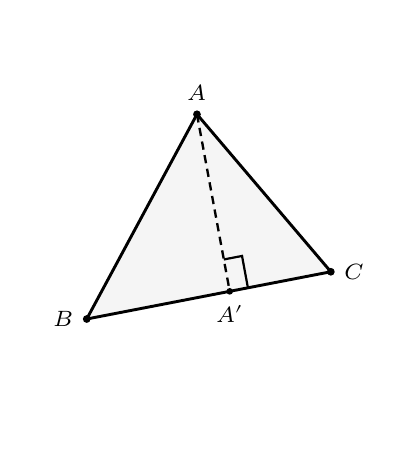
\begin{tikzpicture}[scale=1.00, baseline=(current bounding box.center), every node/.style={font=\footnotesize, text=black}]
    \path (-2.3,-1.65) rectangle (2.3,3.35);
    \coordinate (B) at (-1.55,-0.35);
    \coordinate (C) at (1.55,0.25);
    \coordinate (A) at (-0.15,2.25);
    \coordinate (Ap) at ($(B)!0.5858!(C)$);
    \fill[gray!8] (A) -- (B) -- (C) -- cycle;
    \draw[black, line width=1.05pt] (A) -- (B) -- (C) -- cycle;
    \draw[black, line width=0.85pt, densely dashed] (A) -- (Ap);
    \rightbox[0.18]{A}{Ap}{C}
    \fill[black] (A) circle (1.4pt) node[above=1.5pt] {$A$};
    \fill[black] (B) circle (1.4pt) node[left=1.5pt] {$B$};
    \fill[black] (C) circle (1.4pt) node[right=1.5pt] {$C$};
    \fill[black] (Ap) circle (1.2pt) node[below=1.5pt] {$A'$};
  \end{tikzpicture}
  &
  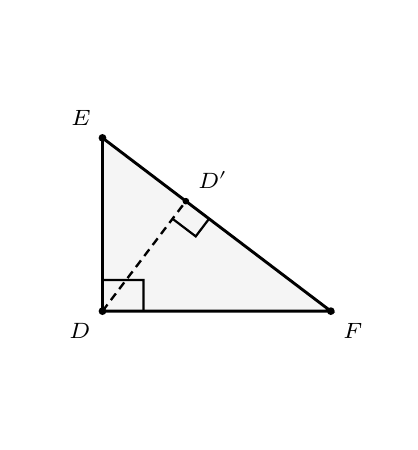
\begin{tikzpicture}[scale=1.00, baseline=(current bounding box.center), every node/.style={font=\footnotesize, text=black}]
    \path (-2.3,-1.65) rectangle (2.3,3.35);
    \coordinate (D) at (-1.35,-0.25);
    \coordinate (F) at (1.55,-0.25);
    \coordinate (E) at (-1.35,1.95);
    \coordinate (Dp) at ($(E)!(D)!(F)$);
    \fill[gray!8] (D) -- (E) -- (F) -- cycle;
    \draw[black, line width=1.05pt] (D) -- (E) -- (F) -- cycle;
    \rightbox[0.18]{E}{D}{F}
    \draw[black, line width=0.85pt, densely dashed] (D) -- (Dp);
    \rightbox[0.16]{D}{Dp}{F}
    \fill[black] (D) circle (1.4pt) node[below left=1pt] {$D$};
    \fill[black] (F) circle (1.4pt) node[below right=1pt] {$F$};
    \fill[black] (E) circle (1.4pt) node[above left=1pt] {$E$};
    \fill[black] (Dp) circle (1.2pt) node[above right=1pt] {$D'$};
  \end{tikzpicture}
  &
  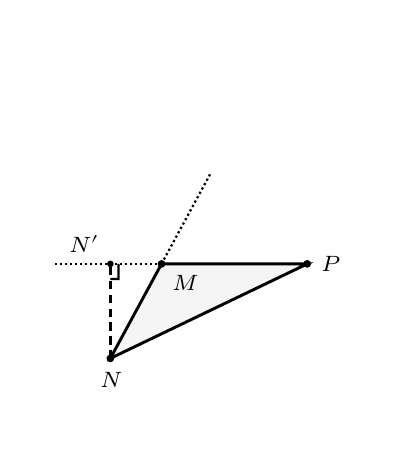
\begin{tikzpicture}[scale=1.00, baseline=(current bounding box.center), every node/.style={font=\footnotesize, text=black}]
    \path (-2.3,-1.65) rectangle (2.3,3.35);
    \coordinate (N) at (-1.25,-0.85);
    \coordinate (M) at (-0.60,0.35);
    \coordinate (P) at (1.25,0.35);
    \coordinate (Np) at (-1.25,0.35);
    \fill[gray!8] (M) -- (N) -- (P) -- cycle;
    \draw[black, line width=1.05pt] (M) -- (N) -- (P) -- cycle;
    \draw[black, line width=0.8pt, densely dotted] (-1.95,0.35) -- (M);
    \draw[black, line width=0.8pt, densely dotted] (M) -- ($(N)!1.95!(M)$);
    \draw[black, line width=0.85pt, densely dashed] (N) -- (Np);
    \rightbox[0.16]{N}{Np}{M}
    \fill[black] (M) circle (1.4pt) node[below right=0.5pt] {$M$};
    \fill[black] (N) circle (1.4pt) node[below=1.5pt] {$N$};
    \fill[black] (P) circle (1.4pt) node[right=1.5pt] {$P$};
    \fill[black] (Np) circle (1.2pt) node[above left=0.5pt] {$N'$};
  \end{tikzpicture} \\
  \hline
  ទីតាំង $H$៖ \chkbox\ ក្នុង \;\chkbox\ កំពូលកែង \;\chkbox\ ក្រៅ &
  ទីតាំង $H$៖ \chkbox\ ក្នុង \;\chkbox\ កំពូល $D$ \;\chkbox\ ក្រៅ &
  ទីតាំង $H$៖ \chkbox\ ក្នុង \;\chkbox\ កំពូល $M$ \;\chkbox\ ក្រៅ \\
  \hline
\end{tabular}}\\[5pt]
$\blacktriangleright$ \textbf{សង្កេតរួម៖} ហេតុអ្វីក្នុងករណីទី៣ (មុំទាល) ចាំបាច់ត្រូវ \textbf{បន្លាយបន្ទាត់ជ្រុងឈម} ជាមុន មុននឹងដាក់អេគែរគូសកម្ពស់? \blank{4.1cm}

\vspace{7pt}
% --- E2 Explore Part B: Auxiliary Triangle PQR Proof ---
\secbar{ផ្នែកទី១ \enbf{(}ខ\enbf{)} ៖ សម្រាយបំភ្លឺតាមត្រីកោណជំនួយ $\tri{PQR}$ \enbf{---} ឧទាហរណ៍ ទំព័រ ២០៨\enbf{--}២០៩}{ការងារជាដៃគូ \en{5 min}}

\noindent
\begin{minipage}[c]{12.3cm}
  $\tri{PQR}$ ជាត្រីកោណមួយ និង $A, B, C$ ជាចំណុចកណ្ដាលនៃជ្រុង $RQ, PR, PQ$ រៀងគ្នា ។ តាង $A', B', C'$ ជាជើងកម្ពស់នៃ $\tri{ABC}$ ។ ចូរបំពេញចន្លោះដើម្បីបង្ហាញថាកម្ពស់ទាំងបីប្រសព្វគ្នាត្រង់ចំណុច $H$ តែមួយ៖\\[4pt]
  $1.$ ដោយ $B$ កណ្ដាល $PR$ និង $C$ កណ្ដាល $PQ$ (បន្ទាត់មធ្យម) $\Longrightarrow BC \parallel \blank{1.3cm}$ ។\\[4pt]
  $2.$ ដោយ $AA' \perp BC$ ហើយ $BC \parallel RQ \Longrightarrow AA' \perp \blank{1.3cm}$ ត្រង់ចំណុច $A$ ។\\[4pt]
  $3.$ តែ $A$ ជាចំណុចកណ្ដាលនៃអង្កត់ $RQ \Longrightarrow$ បន្ទាត់ $AA'$ គឺជា \textbf{\blank{2.2cm}} នៃអង្កត់ $RQ$ ។\\[4pt]
  $4.$ ស្រាយដូចគ្នា បន្ទាត់ $BB'$ និង $CC'$ គឺជា \textbf{\blank{2.2cm}} នៃអង្កត់ $PR$ និង $PQ$ រៀងគ្នា ។\\[4pt]
  $5.$ ដោយមេដ្យាទ័រទាំងបីនៃ $\tri{PQR}$ ប្រសព្វគ្នាត្រង់ចំណុច $H$ តែមួយ នាំឱ្យកម្ពស់ $AA', BB', CC'$ នៃ $\tri{ABC}$ ក៏ប្រសព្វគ្នាត្រង់ចំណុច \blank{0.9cm} តែមួយដែរ (ហៅថា \textbf{\blank{2.4cm}} នៃ $\tri{ABC}$)!
\end{minipage}%
\hfill
\begin{minipage}[c]{6.4cm}
  \centering
  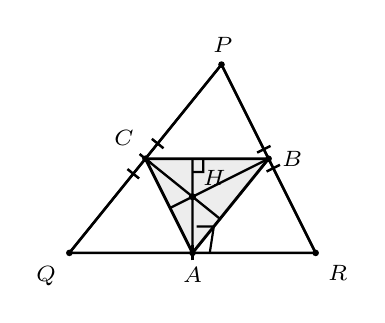
\begin{tikzpicture}[scale=0.92, every node/.style={font=\footnotesize, text=black}]
    \coordinate (A) at (0,-0.85);
    \coordinate (B) at (1.05,0.45);
    \coordinate (C) at (-0.65,0.45);
    \coordinate (P) at (0.40,1.75);
    \coordinate (Q) at (-1.70,-0.85);
    \coordinate (R) at (1.70,-0.85);
    \coordinate (Ap) at (0,0.45);
    \coordinate (Bp) at (-0.31,-0.23);
    \coordinate (Cp) at (0.38,-0.38);
    \coordinate (H) at (0,-0.075);
    \draw[black, line width=0.95pt] (P) -- (Q) -- (R) -- cycle;
    \fill[gray!14] (A) -- (B) -- (C) -- cycle;
    \draw[black, line width=1.05pt] (A) -- (B) -- (C) -- cycle;
    \draw[black, line width=0.85pt] (A) -- (Ap) (B) -- (Bp) (C) -- (Cp);
    \rightbox[0.14]{A}{Ap}{B}
    \rightbox[0.14]{P}{A}{R}
    \draw[black, line width=0.75pt, tk1] (Q) -- (A) (A) -- (R);
    \draw[black, line width=0.75pt, tk2] (P) -- (B) (B) -- (R);
    \draw[black, line width=0.75pt, tk3] (P) -- (C) (C) -- (Q);
    \fill[black] (P) circle (1.3pt) node[above=1pt] {$P$};
    \fill[black] (Q) circle (1.3pt) node[below left=1pt] {$Q$};
    \fill[black] (R) circle (1.3pt) node[below right=1pt] {$R$};
    \fill[black] (A) circle (1.3pt) node[below=1.5pt] {$A$};
    \fill[black] (B) circle (1.3pt) node[right=1.5pt] {$B$};
    \fill[black] (C) circle (1.3pt) node[above left=1pt] {$C$};
    \fill[black] (H) circle (1.4pt) node[above right=0.5pt] {$H$};
  \end{tikzpicture}
\end{minipage}

\vspace{7pt}
% --- E3 Explain: Theorem, Remarks & Warrant Bank ---
\secbar{ផ្នែកទី២ ៖ បញ្ញត្តិទ្រឹស្តីបទ សម្គាល់ និងធនាគារហេតុផល \enbf{(E3 - Explain)}}{សង្ខេបរួមគ្នា \en{6 min}}

\begin{tcolorbox}[
  enhanced, sharp corners, colback=white, colframe=black,
  boxrule=0.9pt, boxsep=3pt, top=4.5pt, bottom=4.5pt, left=6pt, right=6pt
]
  $\bullet$ \textbf{ទ្រឹស្តីបទ (ទំ.២០៩)៖} កម្ពស់ទាំងបីនៃត្រីកោណមួយប្រសព្វគ្នាត្រង់ \textbf{\blank{2.6cm}} ។ ចំណុចប្រសព្វនោះហៅថា \textbf{\blank{2.8cm}} នៃត្រីកោណ ($H$) ។\\[4pt]
  $\bullet$ \textbf{សម្គាល់ (ទំ.២០៩)៖} (១) បើចំណុចមួយនៅលើកម្ពស់ពីរនៃត្រីកោណ វាក៏ឋិតនៅលើ \textbf{\blank{2.4cm}} ដែរ ។ (២) ក្នុងត្រីកោណសម័ង្ស ចំណុចពិសេស $O, G, H$ គឺ \textbf{\blank{2.3cm}} ។\\[4pt]
  $\bullet$ \textbf{ធនាគារហេតុផល៖}
  \cnum{1} និយមន័យកម្ពស់ ($AA'\perp BC$) \;\textbar\;
  \cnum{2} ប្រសព្វកម្ពស់ ២ $\Rightarrow$ កម្ពស់ទី ៣ កាត់តាម $H$ \;\textbar\;
  \cnum{3} ទីតាំង $H$ \;\textbar\;
  \cnum{4} ឯកតាភាពបន្ទាត់កែង \;\textbar\;
  \cnum{5} លក្ខណៈប្រលេឡូក្រាម
\end{tcolorbox}

\newpage

% ============================================================================
% ទំព័រទី ២៖ E4 (លំហាត់គំរូ + ប្រតិបត្តិ) + E5 (ចង្កោមអរតូសង់ #4, #5 & Exit Check) + កិច្ចការផ្ទះ
% ============================================================================

\secbar{ផ្នែកទី៣ ៖ ពង្រីកចំណេះដឹង \enbf{---} លំហាត់គំរូ និងប្រតិបត្តិសៀវភៅគោល \enbf{(E4 - Elaborate)}}{អនុវត្ត \en{10 min}}

\noindent
\begin{minipage}[t]{9.4cm}\vspace{0pt}
  \begin{tcolorbox}[
    enhanced, sharp corners, colback=white, colframe=black, equal height group=rowE4,
    boxrule=0.85pt, boxsep=2.2pt, top=3.5pt, bottom=3.5pt, left=5pt, right=5pt
  ]
    \textbf{៣.ក លំហាត់គំរូ (ទំ.២០៩\,\en{--}\,២១០)៖}\\
    $\tri{ABC}$ និង $\tri{A'BC}$ ជាត្រីកោណកែងពីរមានអ៊ីប៉ូតេនុស $BC$ ដូចគ្នា ។ $I$ ជាចំណុចប្រសព្វនៃបន្ទាត់ $AC$ និង $A'B$ ។ បន្ទាត់កែងនឹង $BC$ កាត់តាម $I$ ជួបបន្ទាត់ $AB$ ត្រង់ $J$ ។ បង្ហាញថា $C, A', J$ រត់ត្រង់ជួរគ្នា៖
    \begin{center}
      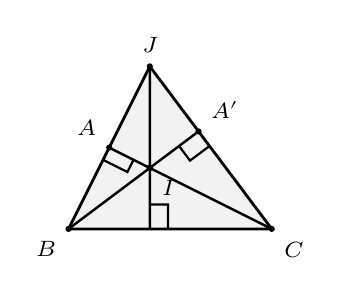
\begin{tikzpicture}[scale=0.86, every node/.style={font=\footnotesize, text=black}]
        \coordinate (B) at (-1.50,-0.65);
        \coordinate (C) at (1.50,-0.65);
        \coordinate (J) at (-0.30,1.75);
        \coordinate (K) at (-0.30,-0.65);
        \coordinate (A) at (-0.90,0.55);
        \coordinate (I) at (-0.30,0.25);
        \coordinate (Ap) at (0.42,0.79);
        \fill[gray!10] (B) -- (C) -- (J) -- cycle;
        \draw[black, line width=1.0pt] (B) -- (C) -- (J) -- cycle;
        \draw[black, line width=0.9pt] (C) -- (A) (B) -- (Ap) (J) -- (K);
        \rightbox[0.15]{C}{A}{B}
        \rightbox[0.15]{B}{Ap}{C}
        \rightbox[0.15]{J}{K}{C}
        \fill[black] (B) circle (1.3pt) node[below left=1pt] {$B$};
        \fill[black] (C) circle (1.3pt) node[below right=1pt] {$C$};
        \fill[black] (J) circle (1.3pt) node[above=1.5pt] {$J$};
        \fill[black] (A) circle (1.3pt) node[above left=1pt] {$A$};
        \fill[black] (Ap) circle (1.3pt) node[above right=1pt] {$A'$};
        \fill[black] (I) circle (1.4pt) node[below right=1pt] {$I$};
      \end{tikzpicture}
    \end{center}
    \vspace{-3pt}
    -- ក្នុងត្រីកោណធំ $\tri{BCJ}$ មាន៖\\
    \hspace*{0.25cm}$\bullet$ $AC \perp BJ$ ត្រង់ $A \Rightarrow CA$ ជា \blank{1.6cm} គូសចេញពីកំពូល $C$ ។\\
    \hspace*{0.25cm}$\bullet$ $JI \perp BC \Rightarrow JI$ ជា \blank{1.6cm} គូសចេញពីកំពូល $J$ ។\\[1.5pt]
    -- ដោយ $I = AC \cap JI \Rightarrow I$ ជា \textbf{\blank{1.9cm}} នៃ $\tri{BCJ}$ (ហេតុផល \blank{0.7cm}) ។\\[1.5pt]
    -- ហេតុនេះ បន្ទាត់ $BI$ (គឺបន្ទាត់ $A'B$) ជាកម្ពស់ទីបី $\Rightarrow A'B \perp \blank{0.9cm}$ ។ តែ $A'B \perp A'C$ ត្រង់ $A'$ (សម្មតិកម្ម) ដូចនេះចំណុច $C, A', J$ \textbf{\blank{2.2cm}}!
  \end{tcolorbox}
\end{minipage}%
\hfill
\begin{minipage}[t]{9.4cm}\vspace{0pt}
  \begin{tcolorbox}[
    enhanced, sharp corners, colback=white, colframe=black, equal height group=rowE4,
    boxrule=0.85pt, boxsep=2.2pt, top=3.5pt, bottom=3.5pt, left=5pt, right=5pt
  ]
    \textbf{៣.ខ ប្រតិបត្តិ (ទំ.២១០)៖ អរតូសង់ឆ្លុះក្នុងប្រលេឡូក្រាម}\\
    ប្រលេឡូក្រាម $ABCD$ មាន $O$ ជាចំណុចប្រសព្វអង្កត់ទ្រូង, $H$ ជាអរតូសង់នៃ $\tri{ABC}$ និង $H'$ ជាអរតូសង់នៃ $\tri{ACD}$ ។ ស្រាយបំភ្លឺថា $O$ ជាចំណុចកណ្ដាលនៃអង្កត់ $HH'$ ៖
    \begin{center}
      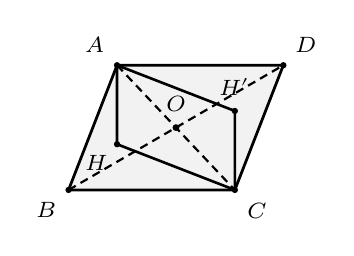
\begin{tikzpicture}[scale=0.88, every node/.style={font=\footnotesize, text=black}]
        \coordinate (O) at (0,0.35);
        \coordinate (A) at (-0.85,1.25);
        \coordinate (B) at (-1.55,-0.55);
        \coordinate (C) at (0.85,-0.55);
        \coordinate (D) at (1.55,1.25);
        \coordinate (H) at (-0.85,0.11);
        \coordinate (Hp) at (0.85,0.59);
        \fill[gray!10] (A) -- (B) -- (C) -- (D) -- cycle;
        \draw[black, line width=1.0pt] (A) -- (B) -- (C) -- (D) -- cycle;
        \draw[black, line width=0.8pt, densely dashed] (A) -- (C) (B) -- (D);
        \draw[black, line width=0.95pt] (A) -- (H) -- (C) -- (Hp) -- cycle;
        \fill[black] (A) circle (1.3pt) node[above left=1pt] {$A$};
        \fill[black] (B) circle (1.3pt) node[below left=1pt] {$B$};
        \fill[black] (C) circle (1.3pt) node[below right=1pt] {$C$};
        \fill[black] (D) circle (1.3pt) node[above right=1pt] {$D$};
        \fill[black] (O) circle (1.4pt) node[above=2pt] {$O$};
        \fill[black] (H) circle (1.3pt) node[below left=0.5pt] {$H$};
        \fill[black] (Hp) circle (1.3pt) node[above=2pt] {$H'$};
      \end{tikzpicture}
    \end{center}
    \vspace{-3pt}
    $1.$ ដោយ $H$ ជាអរតូសង់នៃ $\tri{ABC} \Rightarrow AH \perp BC$ តែ $BC \parallel AD \Rightarrow AH \perp \blank{1.0cm}$ ។ ម្យ៉ាងទៀត $H'$ ជាអរតូសង់នៃ $\tri{ACD} \Rightarrow CH' \perp AD$ នាំឱ្យ $AH \parallel \blank{1.0cm}$ ។\\[2pt]
    $2.$ ដូចគ្នាដែរ $CH \perp AB$ (ហើយ $AB\parallel CD$) និង $AH' \perp CD \Rightarrow CH \parallel \blank{1.0cm}$ ។\\[2pt]
    $3.$ ហេតុនេះ ចតុកោណ $AHCH'$ ជា \textbf{\blank{2.2cm}} ។ ដោយ $O$ ជាចំណុចកណ្ដាលនៃអង្កត់ទ្រូង $AC$ នោះអង្កត់ទ្រូងទីពីរ $HH'$ ក៏មាន $O$ ជា \textbf{\blank{2.2cm}} ដែរ!
  \end{tcolorbox}
\end{minipage}

\vspace{2pt}
% --- E5 Evaluate: Orthocentric System (#4, #5 p.213) + Exit Check ---
\secbar{ផ្នែកទី៤ ៖ វាយតម្លៃលទ្ធផលសិក្សា \enbf{---} លំហាត់ទី៤ និងទី៥ \enbf{(}ទំ\enbf{.}២១៣\enbf{)} និងសំណួរត្រួតពិនិត្យរហ័ស \enbf{(E5)}}{ធ្វើដោយឯករាជ្យ \en{10 min}}

\noindent
\begin{minipage}[t]{10.2cm}\vspace{0pt}
  \begin{tcolorbox}[
    enhanced, sharp corners, colback=white, colframe=black, equal height group=rowE5,
    boxrule=0.85pt, boxsep=2.2pt, top=3.5pt, bottom=3.5pt, left=5pt, right=5pt
  ]
    \textbf{៤.ក ចង្កោមអរតូសង់ និងការកំណត់ប្រភេទត្រីកោណ (ទំ.២១៣)៖}\\[2.5pt]
    \textbf{១. លំហាត់ទី៤ (ទំ.២១៣)៖} គេឱ្យ $H$ ជាអរតូសង់នៃត្រីកោណមុំស្រួច $\tri{ABC}$ ($AH\perp BC,\; BH\perp AC,\; CH\perp AB$) ។ ចូរបញ្ជាក់ប្រាប់អរតូសង់នៃត្រីកោណខាងក្រោម៖\\[3pt]
    \hspace*{0.15cm}$\bullet$ ក្នុង $\tri{ABH}$៖ $AC\perp BH$ និង $BC\perp AH \Rightarrow$ អរតូសង់គឺកំពូល \blank{0.9cm}\\[3pt]
    \hspace*{0.15cm}$\bullet$ ក្នុង $\tri{CAH}$៖ $BA\perp CH$ និង $BC\perp AH \Rightarrow$ អរតូសង់គឺកំពូល \blank{0.9cm}\\[3pt]
    \hspace*{0.15cm}$\bullet$ ក្នុង $\tri{BCH}$៖ $AB\perp CH$ និង $AC\perp BH \Rightarrow$ អរតូសង់គឺកំពូល \blank{0.9cm}\\[4pt]
    \textbf{២. លំហាត់ទី៥ (ទំ.២១៣)៖} បើអរតូសង់ $H$ នៃ $\tri{ABC}$ ឋិតនៅលើមេដ្យាទ័រនៃអង្កត់ $BC$ នោះកម្ពស់គូសពី $A$ ត្រួតស៊ីគ្នានឹងមេដ្យាទ័រនៃ $BC$ ។\\[2pt]
    $\Rightarrow$ ដូចនេះ $\tri{ABC}$ គឺជាត្រីកោណ \blank{4.5cm} ។
  \end{tcolorbox}
\end{minipage}%
\hfill
\begin{minipage}[t]{8.6cm}\vspace{0pt}
  \begin{tcolorbox}[
    enhanced, sharp corners, colback=white, colframe=black, equal height group=rowE5,
    boxrule=0.85pt, boxsep=2.2pt, top=3.5pt, bottom=3.5pt, left=5pt, right=5pt
  ]
    \textbf{៤.ខ សំណួរត្រួតពិនិត្យរហ័ស (\en{Exit Check})៖}\\
    ចូរគូសវង់ជុំវិញអក្សរនៃចម្លើយត្រឹមត្រូវតែមួយគត់៖\\[3.5pt]
    \textbf{សំណួរទី១៖} បើ $\tri{ABC}$ ជាត្រីកោណកែងត្រង់កំពូល $A$ តើអរតូសង់ $H$ ស្ថិតនៅត្រង់ណា?\\
    \hspace*{0.15cm}\textbf{ក.} ត្រង់កំពូលមុំកែង $A$ \hspace{0.45cm}
    \textbf{ខ.} ចំណុចកណ្ដាលនៃ $BC$\\
    \hspace*{0.15cm}\textbf{គ.} ខាងក្រៅត្រីកោណ \hspace{0.55cm}
    \textbf{ឃ.} ទីប្រជុំទម្ងន់ $G$\\[4.5pt]
    \textbf{សំណួរទី២ (បេសកកម្ម E1)៖} ចំពោះត្រីកោណមុំទាល តើអរតូសង់ $H$ ស្ថិតនៅត្រង់ណា?\\
    \hspace*{0.15cm}\textbf{ក.} ខាងក្នុងត្រីកោណ \hspace{0.62cm}
    \textbf{ខ.} កណ្ដាលជ្រុងវែងជាងគេ\\
    \hspace*{0.15cm}\textbf{គ.} ខាងក្រៅត្រីកោណ \hspace{0.55cm}
    \textbf{ឃ.} មិនប្រសព្វគ្នាទេ\\[4.5pt]
    \textbf{សំណួរទី៣៖} ក្នុងត្រីកោណប្រភេទណាដែល $O, G$ និង $H$ ត្រួតស៊ីគ្នាតែមួយ?\\
    \hspace*{0.15cm}\textbf{ក.} ត្រីកោណកែង \hspace{0.6cm} \textbf{ខ.} ត្រីកោណសម័ង្ស
  \end{tcolorbox}
\end{minipage}

\vspace{2pt}
% --- Step 5 Homework Box ---
\secbar{ផ្នែកទី៥ ៖ កិច្ចការផ្ទះ និងការរៀបចំមេរៀនបន្ទាប់ \enbf{(}សៀវភៅគោល ទំព័រ ២១៤\enbf{)}}{ធ្វើនៅផ្ទះក្នុងសៀវភៅសរសេរ}

\begin{tcolorbox}[
  enhanced, sharp corners, colback=panelgray, colframe=black,
  boxrule=0.85pt, boxsep=2.5pt, top=3.5pt, bottom=3.5pt, left=6pt, right=6pt
]
  $1.$ \textbf{លំហាត់ទី៩ (ទំ.២១៤)៖} ក្នុងប្រលេឡូក្រាម $ABCD$ បន្ទាត់កែងនឹង $BC$ តាម $A$ និងបន្ទាត់កែងនឹង $AC$ តាម $B$ ប្រសព្វគ្នាត្រង់ $E$ ។ ប្រាប់ប្រភេទនៃត្រីកោណ $\tri{CDE}$ ។\\[2.5pt]
  $2.$ \textbf{លំហាត់ទី១០ និងទី១១ (ទំ.២១៤)៖} (ក) $\tri{ABC}$ កែងត្រង់ $A$, $D$ ជើងកម្ពស់ពី $A$, $I$ កណ្ដាល $BD$, $J$ កណ្ដាល $AD$ ។ ស្រាយបំភ្លឺថា $AI \perp CJ$ \textit{(តម្រុយ៖ ពិនិត្យបន្ទាត់មធ្យម $IJ\parallel AB$ នាំឱ្យ $J$ ជាអរតូសង់នៃ $\tri{ACI}$!)} ។ (ខ) សរសេរសម្រាយពេញលេញនៃលំហាត់ទី១១ ($O$ កណ្ដាល $HH'$) ។\\[2.5pt]
  $3.$ \textbf{កិច្ចការអានជាមុន៖} អានចំណុច \textbf{១៦.៤ លក្ខណៈកន្លះបន្ទាត់ពុះមុំនៃត្រីកោណ} (ទំ.២១០\,\en{--}\,២១១) និងត្រៀមដែកឈាន រ៉ាប់ព័រទ័រ អេគែរ ។
\end{tcolorbox}

\end{document}
